In diesem Versuch wird der Faraday-Effekt verwendet, um die effektive Masse von
Galliumarsenid zu bestimmen. Hierfür werden zwei n-dotierte und eine undotierte
Proben des Halbleiters verwendet.

\section{Theorie}
\label{sec:Theorie}

\subsection{Effektive Masse}\label{sec:effektive_masse}
Die Energieniveaus der einzelnen Atome in einem Kristall überlagern sich und es ensteht eine komplexe Bandstruktur.
Hierdurch gestaltet sich eine exakte mathemaische Beschreibung meist schwierig und es bedarf
einer Approximation.
Bei Halbleitern eignet als Approximationen, die Betrachtung des Leitungsbandes um das Minimum herum (siehe Abb. \ref{fig:band}).
\begin{figure}
\centering
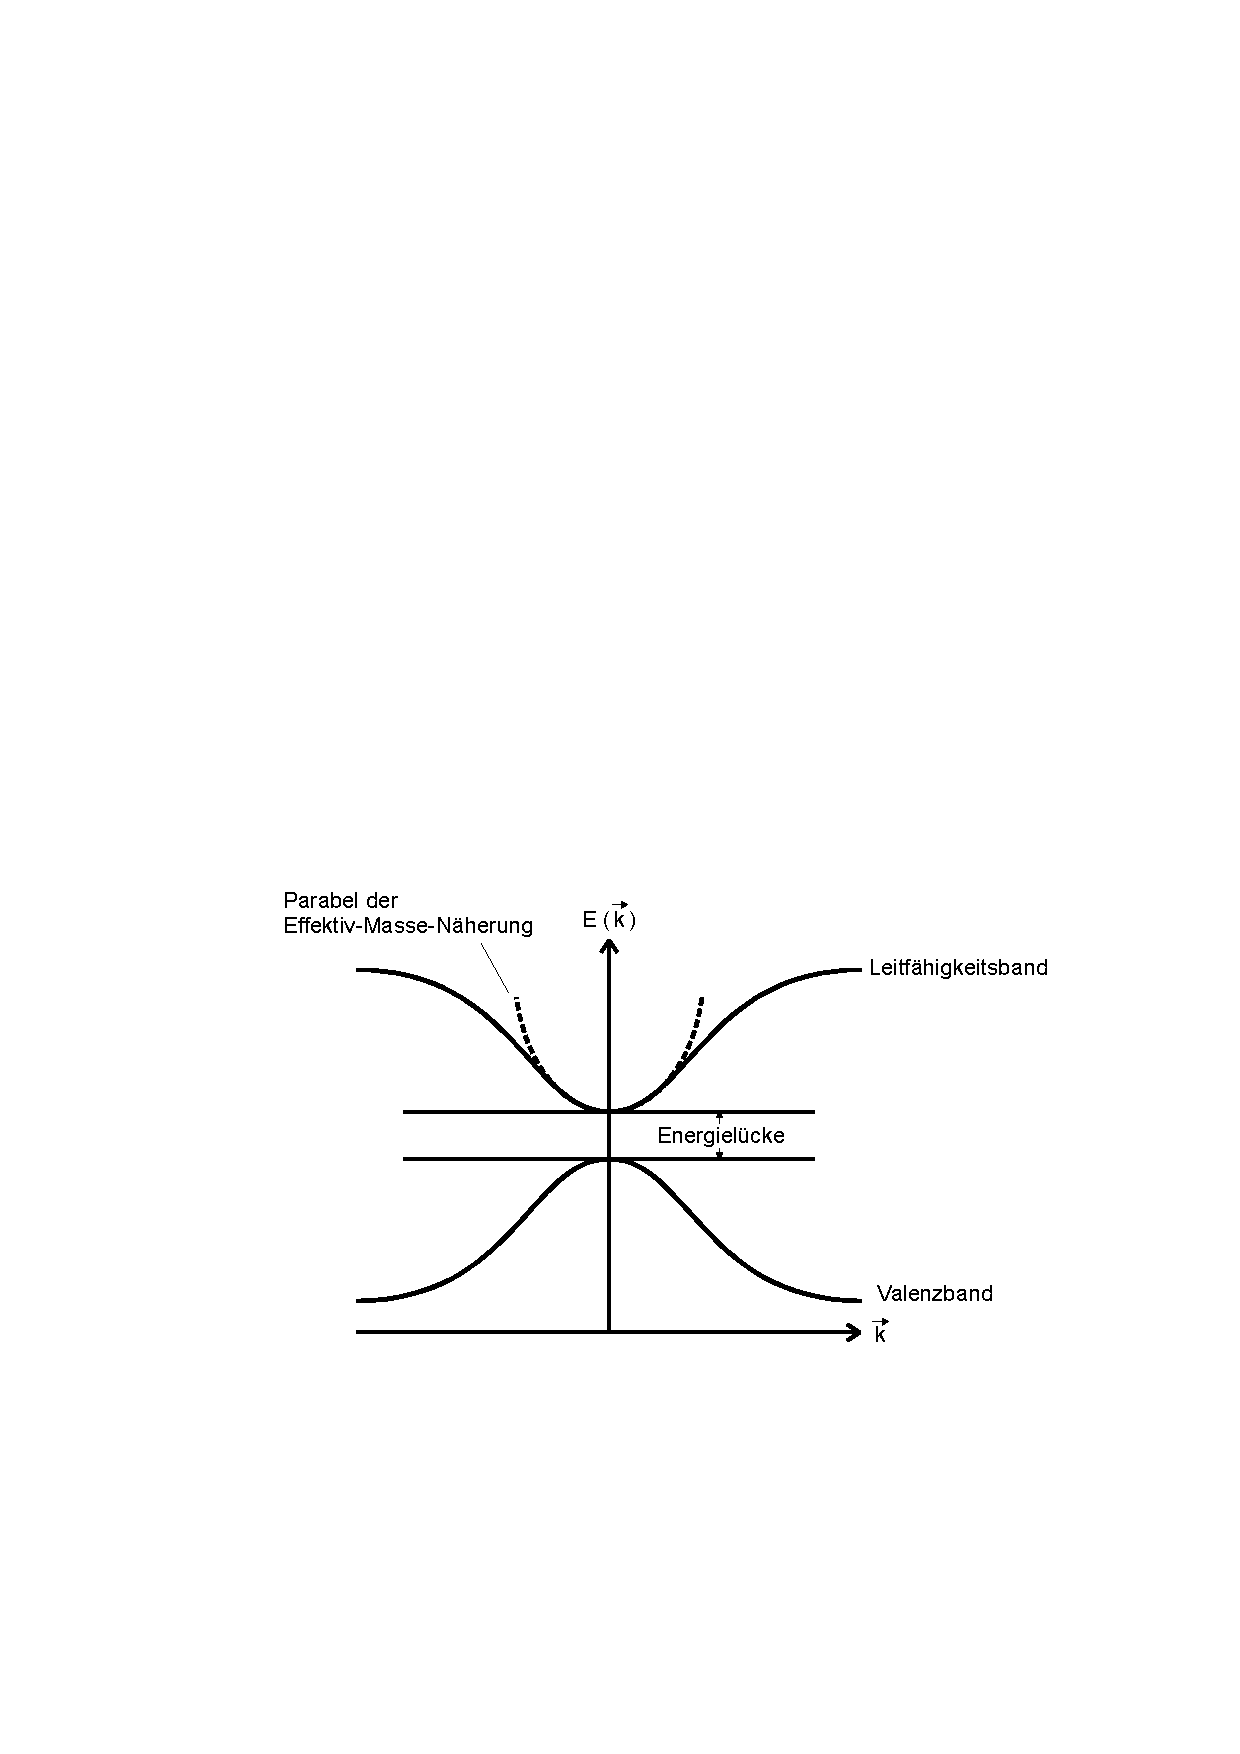
\includegraphics[width=0.5\linewidth]{./content/images/band.pdf}
\caption{Approximationen der Bandstruktur im Halbleiter.}
\label{fig:band}
\end{figure}
In der Umgebung um das Minimum kann die Energie des Bandes $\varepsilon$
in Abhängigkeit mit dem Wellenzahlvektor $\vec{k}$ genährt werden als:
\begin{equation}
  \label{eq:gleichung_energie}
  \varepsilon(\vec{k})=\varepsilon(0) + \frac{1}{2}\sum_{i=1}^3 \left.\frac{\partial^2 \varepsilon}{\partial k_i^2}\right|_{k=0}k_i^2 + \mathcal{O}(k^3)
\end{equation}
Dieser Term ermöglicht die Einführung der effektiven Masse
\begin{equation}
  \label{eq:effetive_masse}
  m^{*}_i := \frac{\hbar^2}{\left.\frac{\partial^2 \varepsilon}{\partial k_i^2}\right|_{k=0}}.
\end{equation}
Der Vorteil, in der Verwendung der effektiven Masse, liegt in der Tatsache, dass
die Definition \eqref{eq:effetive_masse} die Periodizität des Kristallpotentials
$V(\vec{r})$ mitberücksichtigt.
Dadurch kann der Hamilton Operator für ein Kristallelektron,
mit Hilfe der effektiven Masse, in einen Hamilton Operator für ein freies
Teilchen überführt werden:
\begin{equation*}
  \hat{H}:\quad \frac{\hbar^2}{2m_e}\nabla^2 + V(\vec{r}) \quad \rightarrow \quad   \frac{\hbar^2}{2m^*}\nabla^2
\end{equation*}
Ein weiterer Vorteil in der Beschreibung der Dynamik mit der effektiven Masse ist,
dass eine klassische newtonsche Betrachtung möglich ist unter der Voraussetzung eines kleinen
externen elektrischen und magnetischen Feldes.
Diese Eigenschaft wird insbesondere im übernächsten Kapitel von Nutzen sein.

\subsection{Zirkulare Doppelbrechung}
Wird die Polarisationsebene von linear polarisiertes Licht $E(z)$ bei der Propagation
durch einen Kristall der Länge $L$ gedreht, wird dies als zirkulare Doppelbrechung bezeichnet (vgl. Abb. \ref{fig:zirkulare_doppelbrechung}).
\begin{figure}
\centering
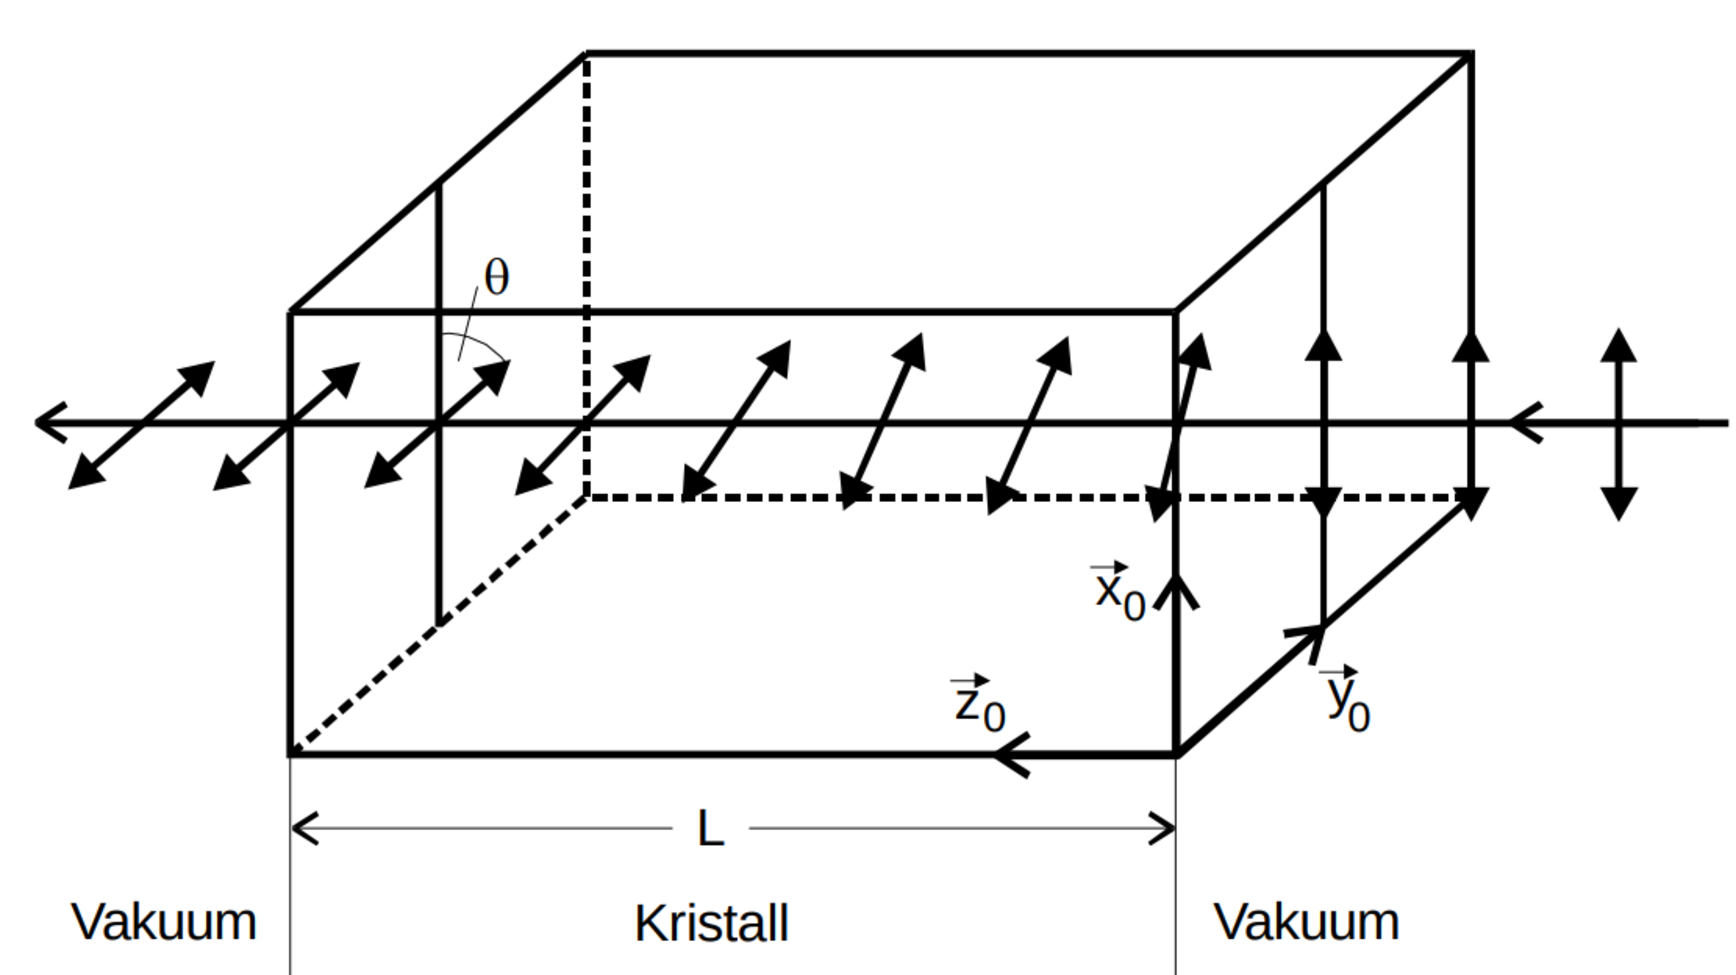
\includegraphics[width=0.5\linewidth]{./content/images/drehung_polarisationsebene.pdf}
\caption{Schmeatische Darstellung von zirkularer Doppelbrechung.}
\label{fig:zirkulare_doppelbrechung}
\end{figure}
Phänomenologisch erklären lässt sich dieser Effekt durch die Annahme, dass sich im
Kristall die Phasengeschwindigkeit für links- und rechtszirkular polarisiertes
Licht $E_\text{L}, E_\text{R}$ unterscheiden.
Diese Eigenschaft wirkt sich auf die Polarisationsebene
von linear polarisiertem Licht aus, da dieses als Linearkombination
von links- und rechtszirkularen Anteilen dargestellt werden kann:
\begin{equation}
  \label{eq:superpos_linear}
\vec{E}(z) = \frac{1}{2}( \vec{E}_\text{R}(z) + \vec{E}_\text{L}(z)), \quad k_\text{R}\neq k_\text{L}
\end{equation}
Wobei die links- und rechtszirkularen Felder definiert sind als
\begin{align}
  \label{eq:def_rechts_links}
  \begin{aligned}
  \vec{E}_\text{R}(z) &= \left(E_0 \vec{x}_0 - \text{i}E_0\vec{y}_0\right)\exp\left(\text{i}{k}_\text{R}z\right)\\
  \vec{E}_\text{L}(z) &= \left(E_0 \vec{x}_0 + \text{i}E_0\vec{y}_0\right)\exp\left(\text{i}{k}_\text{L}z\right).
\end{aligned}
\end{align}
Die Defintionen \eqref{eq:def_rechts_links} werden in die Gleichung \eqref{eq:superpos_linear}
eingesetzt.
Zusätzlich werden die Winkel
\begin{align}
  \label{eq:winkel}
  \begin{aligned}
    \Psi&:=\frac{L}{2}(k_\text{R}+k_\text{L}) \\
    \vartheta &:= \frac{L}{2}(k_\text{R}-k_\text{L}) \overset{k_i=\frac{n_i\omega}{\text{c}_0}}{=} \frac{L\omega}{2\text{c}_0}\left(n_\text{R}-n_\text{L}\right)
\end{aligned}
\end{align}
eingeführt mit dem jeweilige Brechungsindex $n$.
Nach einer kurzen Rechnung ergibt sich ein
Ausdruck für das aus dem Kristall austretende Licht:
\begin{equation*}
  \vec{E}(L)=E_0 \exp(\text{i}\Psi)\left(\cos(\vartheta) \vec{x}_0 + \sin(\vartheta)\vec{y}_0\right)
\end{equation*}

Eine präzisere Beschreibung der zirkularen Doppelbrechung ist durch induzierte
Dipole im Kristall möglich.
Die Dipole erzeugen eine Polarisation $\vec{P}$ des Kristalls,
die für kleine elektrische Felder formuliert werden kann als
\begin{equation*}
\vec{P}=\varepsilon_0\chi\vec{E}.
\end{equation*}
Hierbei ist $\varepsilon_0$ die Influenzkonstante und $\chi$ die
dielektrische Suszeptibilität, welche in anistropen Kristallen als
Tensor $\overline{\overline{chi}}$ geschrieben wird.
Doppelbrechung entsteht genau dann, wenn ein Kristall anistrope Eigenschaften aufweist.
Der Beweis dieser Behauptung wird im Folgenden skizziert.
Hierfür wird die folgende dielektrische Suszeptibilität
 $\overline{\overline{chi}}$ betrachtet:
\begin{equation}
  \label{eq:chi_tens_example}
  \overline{\overline{chi}}=\begin{pmatrix} \chi_\text{xx} & \text{i}\chi_\text{xy} & 0 \\ -\text{i}\chi_\text{yx} & \chi_\text{xx} & 0 \\ 0 & 0 & \chi_\text{zz} \end{pmatrix}.
\end{equation}
Propagiert ein elektrisches Feld durch Materie, so erfolgt die Änderung des Feldes nach:
\begin{equation}
  \label{eq:e_feld_in_materie}
  \vec{D}=\varepsilon_0\left(1+\overline{\overline{chi}}\right)\vec{E}.
\end{equation}
Wird nun die Gleichung \eqref{eq:e_feld_in_materie} mit \eqref{eq:chi_tens_example}
in die homogene Wellengleichung
\begin{equation*}
  \Box \vec{D} = 0
\end{equation*}
eingesetzt, ergbit sich nach einer etwas längeren Rechnung,
dass die Drehung der Polarisationsebene $\vartheta$ gegeben ist durch:
\begin{equation}
  \label{eq:drehung_mit_chi}
  \vartheta \approx \frac{L\omega}{2\text{c}_0} \frac{1}{\sqrt{1+\chi_\text{xx}}} \chi_{xy}\approx \frac{L\omega}{2\text{c}_0n} \chi_\text{xy}.
\end{equation}
Bei der Herleitung der Gleichung \eqref{eq:drehung_mit_chi}, wurde unter anderem angenommen,
dass sich die Welle in $z$-Richtung ausbreitet ($\vec{k}=k\vec{z}_0$).

\subsection{Faraday-Effekt}
Der Faraday-Effekt beschreibt das Phänomen, dass ein optisches
Medium, durch ein externes Magnetfeld, Nebendiagnonalelemente im elektrischen Suszeptibilitättensor erhält.
Hierdurch wird die Polarisationsebene eines Lichtfeldes $\vec{E}$ gedreht, das parallel zum Magnetfeld einfällt.
Dieses Phänomen kann präziser erfasst werden, durch die Betrachtung von gebunden Elektronen im Magnetfeld $\vec{B}$, welche zusätzlich durch ein elektrisches Feld (verursacht durch die Lichtwelle) gestört werden.
\begin{equation}
  \label{eq:klassische_Bewegungsgleichung}
  m\ddot{\vec{r}}+K\vec{r}=-\text{e}\vec{E}(\vec{r})_0-\text{e}\dot{\vec{r}}\times\vec{B}
\end{equation}
Der Vektor $\vec{r}$ bezeichnet die Auslenkung des Elektrons aus der Gleichgewichtslage, die Konstante $K$ bezeichnet die Bindung des Elektrons an seine Umgebung, die Elementarladung
ist gegeben durch $\text{e}_0$ und die Feldstärke der einfallenden Lichtwelle
wird durch $\vec{E}$ repräsentiert.
Unter der Annahme quasifreier Ladungsträger kann
aus der Differntialgleichung \eqref{eq:klassische_Bewegungsgleichung} ein Ausdruck
für den Drehwinkel der Polarisationsebene $\vartheta$ abgeleitet werden:
\begin{equation}
  \label{eq:drehwinkel}
  \frac{\vartheta}{L}\approx \frac{\text{e}^3\lambda^2 NB}{8\pi^2\varepsilon_0\text{c}_0^3}\frac{1}{m^2} = \frac{\text{e}^3\lambda^2 NB}{8\pi^2\varepsilon_0\text{c}_0^3}\frac{1}{m^{*2}}
\end{equation}
Das Ersetzen von $m$ durch $m^*$ ist durch die in Abschnitt \ref{sec:effektive_masse}
besprochene Eigenschaft der effektiven Masse gerechtfertigt.
Der Drehwinkel $\vartheta$ hängt daraus folgend mit der Ladungsträgerzahl $N$ und dem Magnetfeldstärke $B$ zusammen.
